% !TEX TS-program = XeLaTeX
% !TEX encoding = UTF-8 Unicode

%%%%%%%%%%%%%%%%%%%%%%%%%%%%%%%%%%%%%%%%%%%%%%%%%%%%%%%%%%%%%%%%%%%%%%
%
%  哈尔滨工程大学学位论文 XeLaTeX 模版 —— 作者介绍 resume.tex
%
%  版本:1.0.0
%  最后更新:
%  修改者:Leo LiWenhui lwh@hrbeu.edu.cn
%  修订者:
%  编译环境1:Ubuntu 12.04 + TeXLive 2013/2014
%  编译环境2:Windows 7/8  + TeXLive 2013/2014
%
%%%%%%%%%%%%%%%%%%%%%%%%%%%%%%%%%%%%%%%%%%%%%%%%%%%%%%%%%%%%%%%%%%%%%

\appendix{作者简介}

\begin{window}[0,r,{\mbox{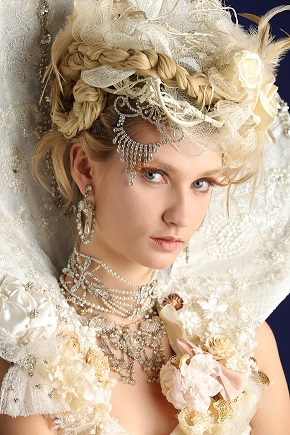
\includegraphics[width=3.5cm]{author.jpg}}},{}]
\end{window}

姓名:张 三

性别:男

出生年月:1985~年~00~月~00~日

民族:汉

籍贯:上海市

研究方向:图形图像处理

简历:

从这里开始写简历

200X.9-200X.7  XX大学XX专业个人简历,从大学起。

200X.9-200X.7  XX大学XX专业个人简历,从大学起。

200X.9-200X.7  XX大学XX专业个人简历,从大学起。

200X.9-200X.7  XX大学XX专业个人简历,从大学起。

200X.9-200X.7  XX大学XX专业个人简历,从大学起。
